% Standalone document to compose gallery figure from 10processor images
\documentclass[multi=tabular, border=4pt]{standalone}
\usepackage{graphicx}
\usepackage{array}
\usepackage{makecell}
\graphicspath{{10processor/}{figures/10processor/}}

\newcommand{\rowlab}[2]{\smash{\makecell[r]{\fontsize{5}{5.2}\selectfont\sffamily #1\\[-0.6pt]\fontsize{4}{4.2}\selectfont\sffamily #2}}}
\newcommand{\collab}[1]{{\tiny\sffamily\bfseries #1}}

\begin{document}
\begin{tabular}{r@{\hspace{4pt}}c@{\hspace{3pt}}c@{\hspace{3pt}}c@{\hspace{3pt}}c}
& \collab{$\gamma = 0.2$} & \collab{$\gamma = 0.4$} & \collab{$\gamma = 0.8$} & \collab{$\gamma = 1.0$} \\[2pt]
\rowlab{1-block}{No AdaIN} &

\includegraphics[width=2.0cm]{proc01_adainfalse_gamma0.2.png} &

\includegraphics[width=2.0cm]{proc01_adainfalse_gamma0.4.png} &

\includegraphics[width=2.0cm]{proc01_adainfalse_gamma0.8.png} &

\includegraphics[width=2.0cm]{proc01_adainfalse_gamma1.png} \\[1pt]
\rowlab{1-block}{AdaIN} &

\includegraphics[width=2.0cm]{proc01_adaintrue_gamma0.2.png} &

\includegraphics[width=2.0cm]{proc01_adaintrue_gamma0.4.png} &

\includegraphics[width=2.0cm]{proc01_adaintrue_gamma0.8.png} &
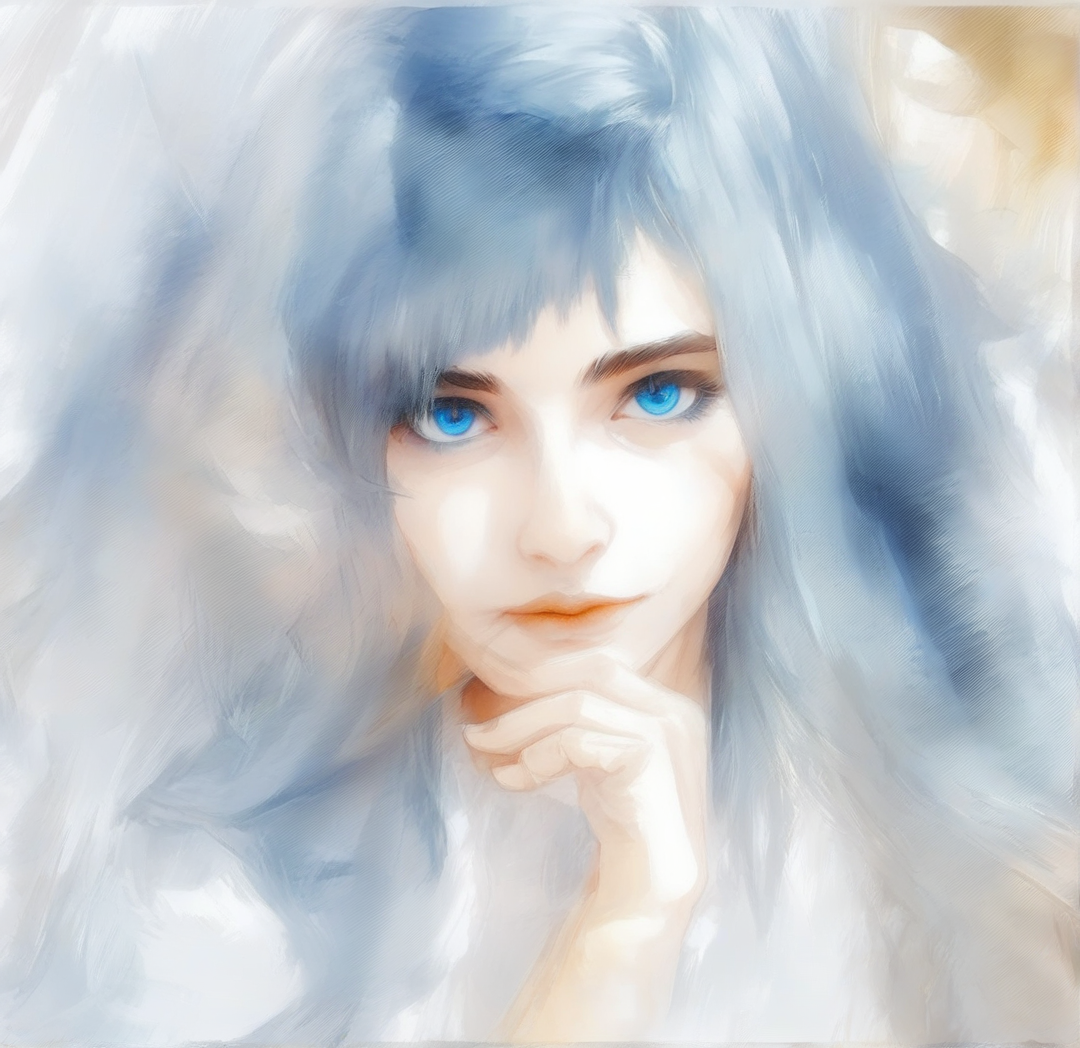
\includegraphics[width=2.0cm]{proc01_adaintrue_gamma1.png} \\[1pt]
\rowlab{5-block}{No AdaIN} &

\includegraphics[width=2.0cm]{proc05_adainfalse_gamma0.2.png} &

\includegraphics[width=2.0cm]{proc05_adainfalse_gamma0.4.png} &

\includegraphics[width=2.0cm]{proc05_adainfalse_gamma0.8.png} &
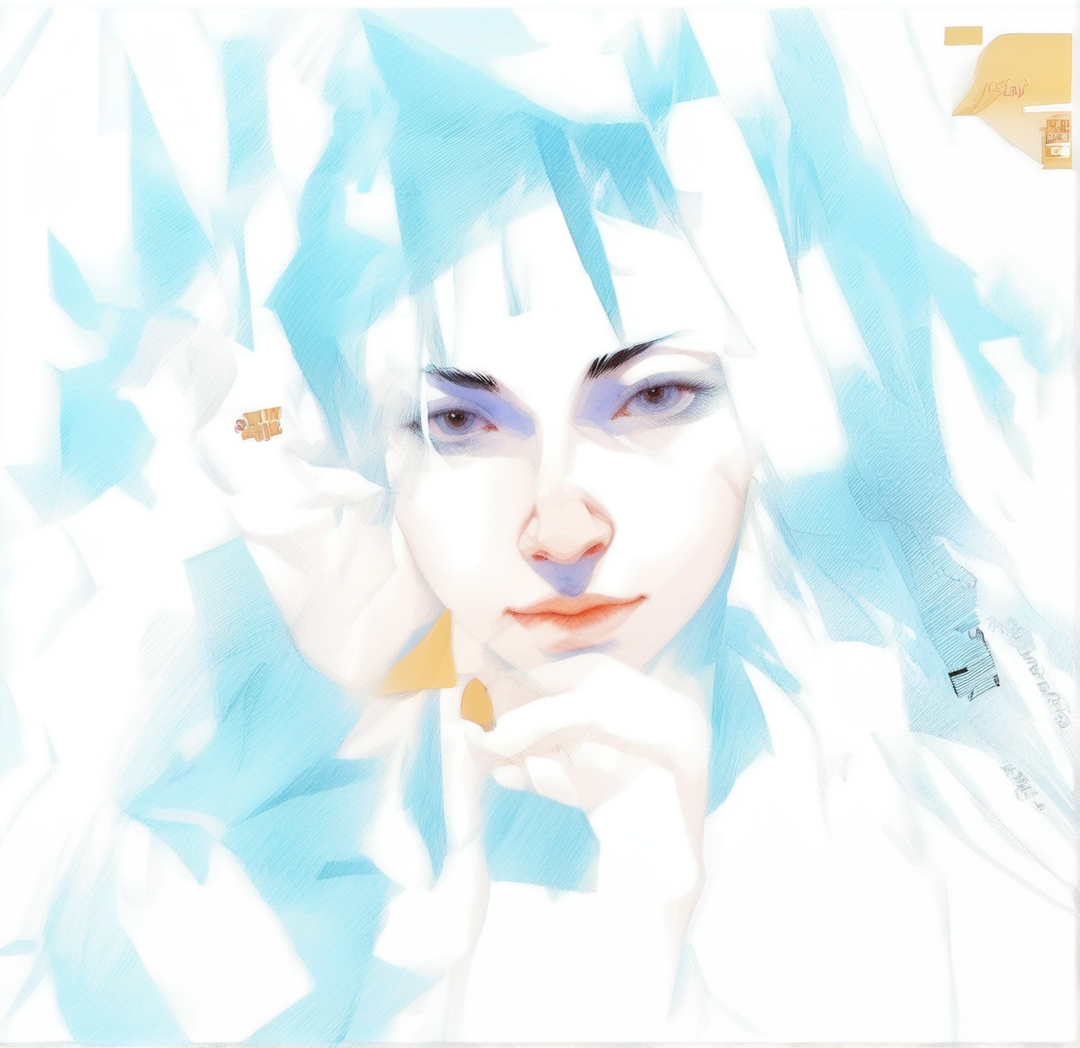
\includegraphics[width=2.0cm]{proc05_adainfalse_gamma1.png} \\[1pt]
\rowlab{5-block}{AdaIN} &
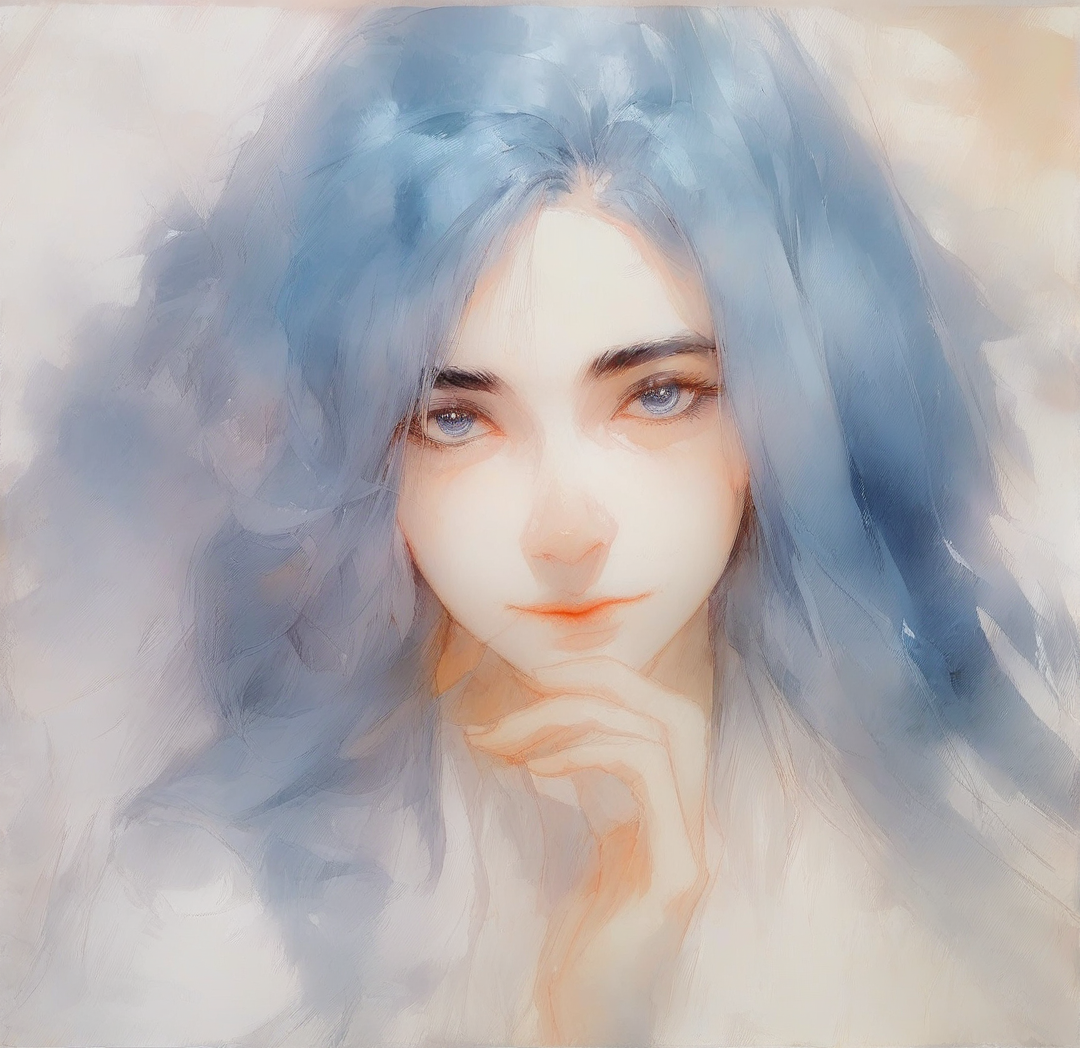
\includegraphics[width=2.0cm]{proc05_adaintrue_gamma0.2.png} &
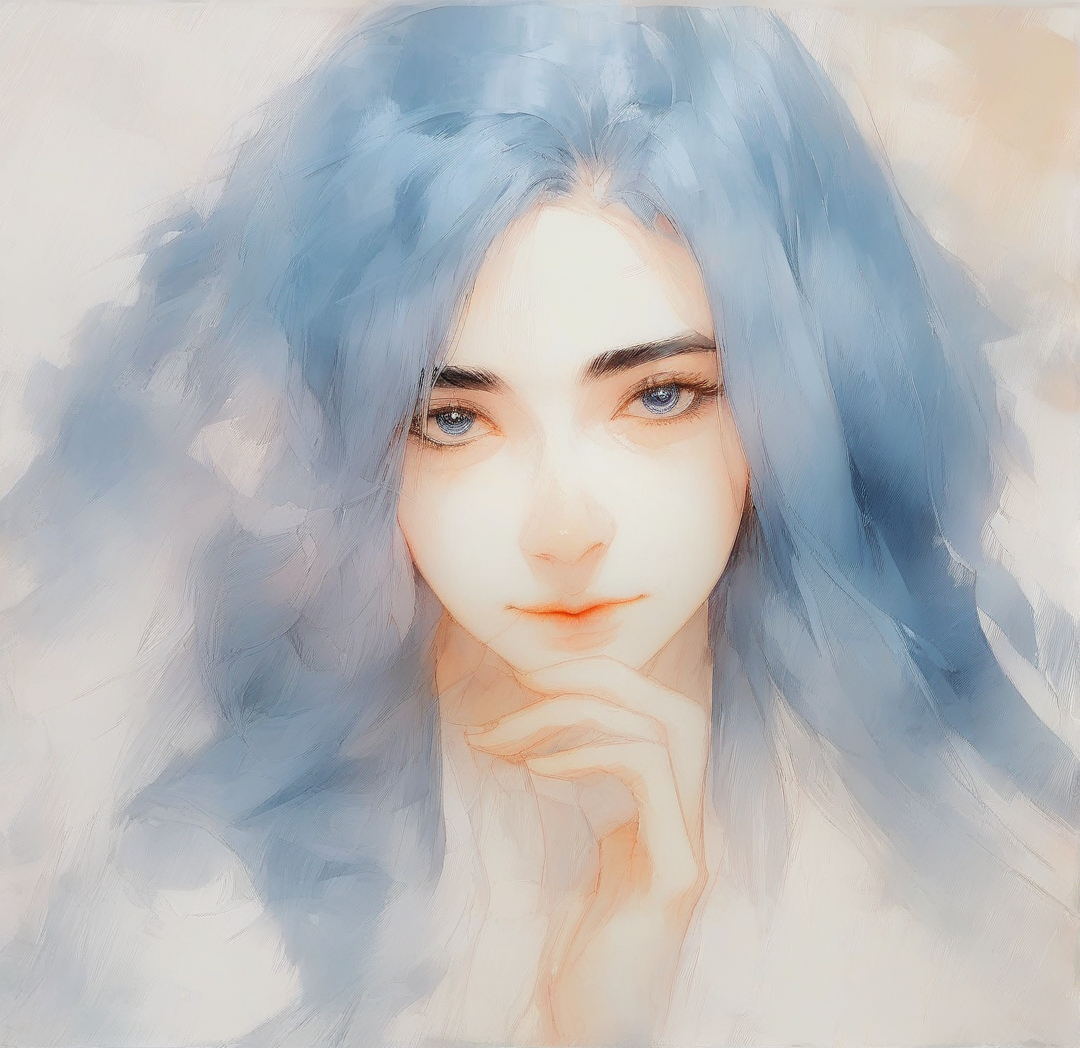
\includegraphics[width=2.0cm]{proc05_adaintrue_gamma0.4.png} &
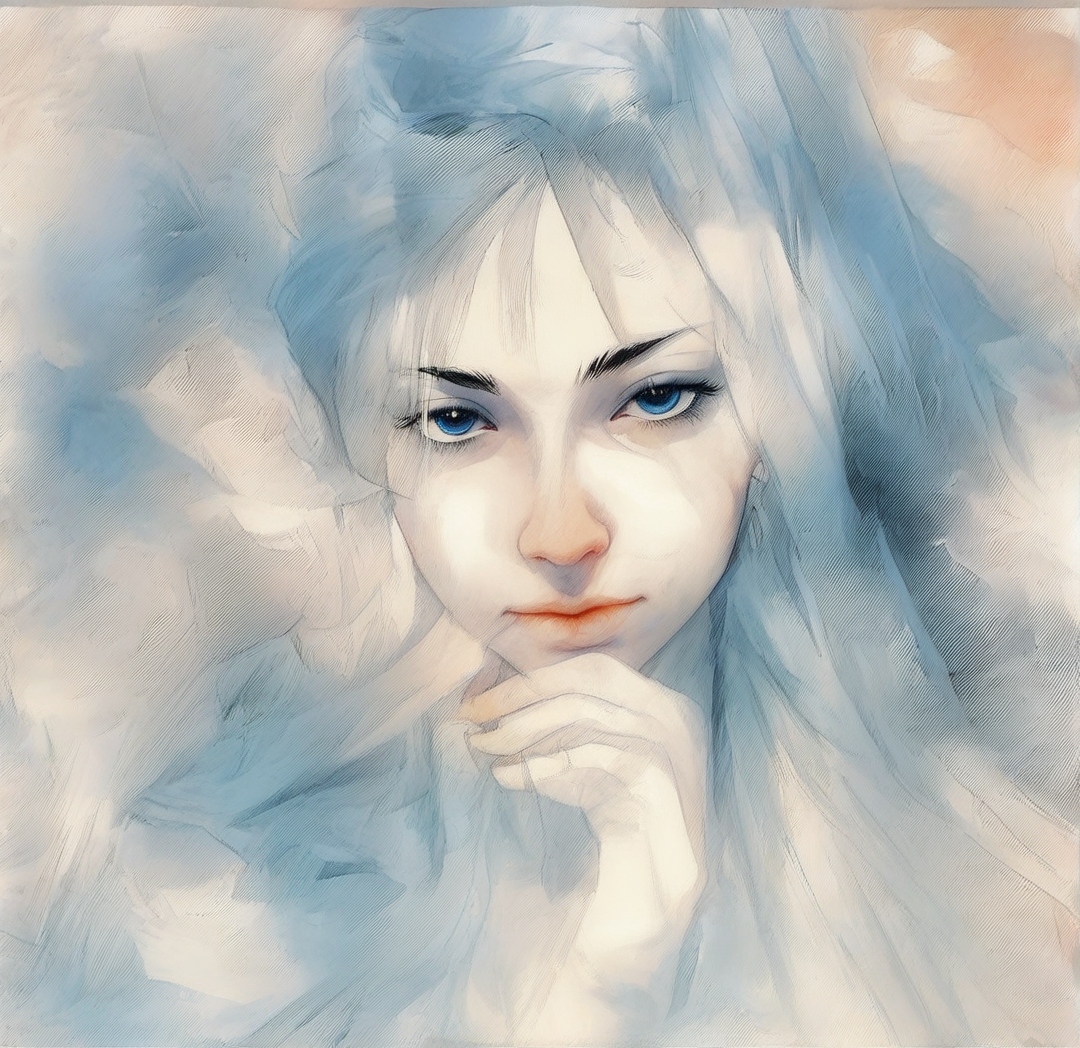
\includegraphics[width=2.0cm]{proc05_adaintrue_gamma0.8.png} &
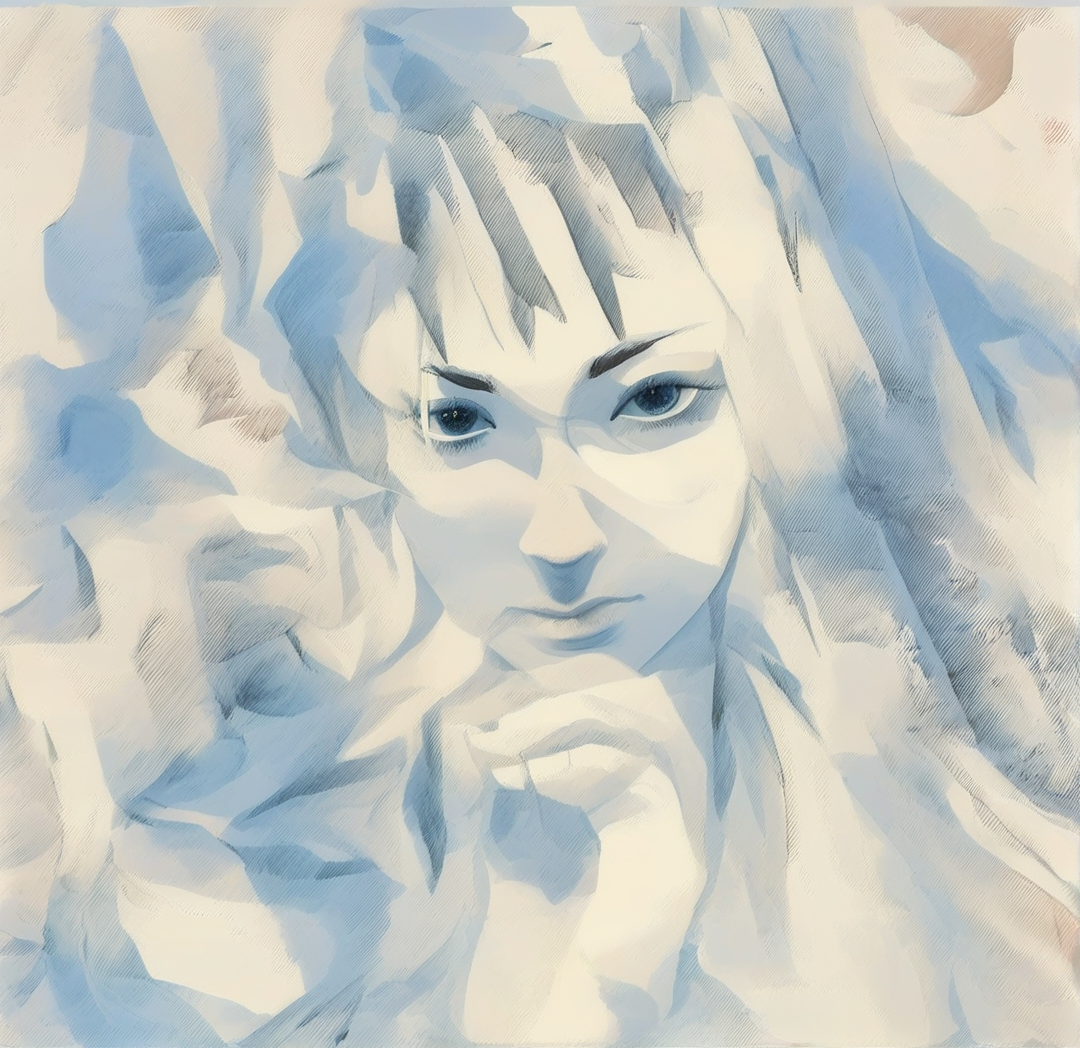
\includegraphics[width=2.0cm]{proc05_adaintrue_gamma1.png} \\[1pt]
\rowlab{10-block}{No AdaIN} &

\includegraphics[width=2.0cm]{proc10_adainfalse_gamma0.2.png} &

\includegraphics[width=2.0cm]{proc10_adainfalse_gamma0.4.png} &
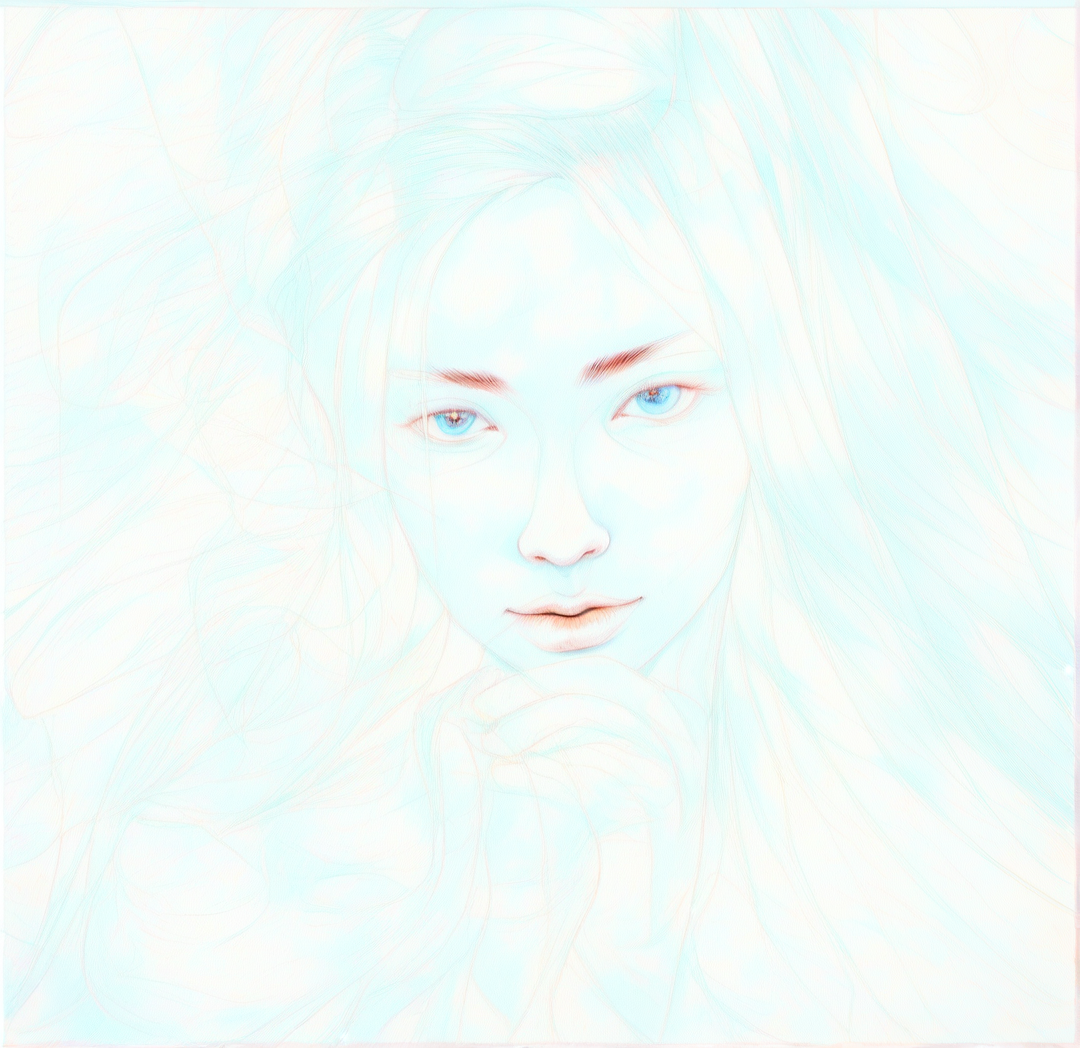
\includegraphics[width=2.0cm]{proc10_adainfalse_gamma0.8.png} &
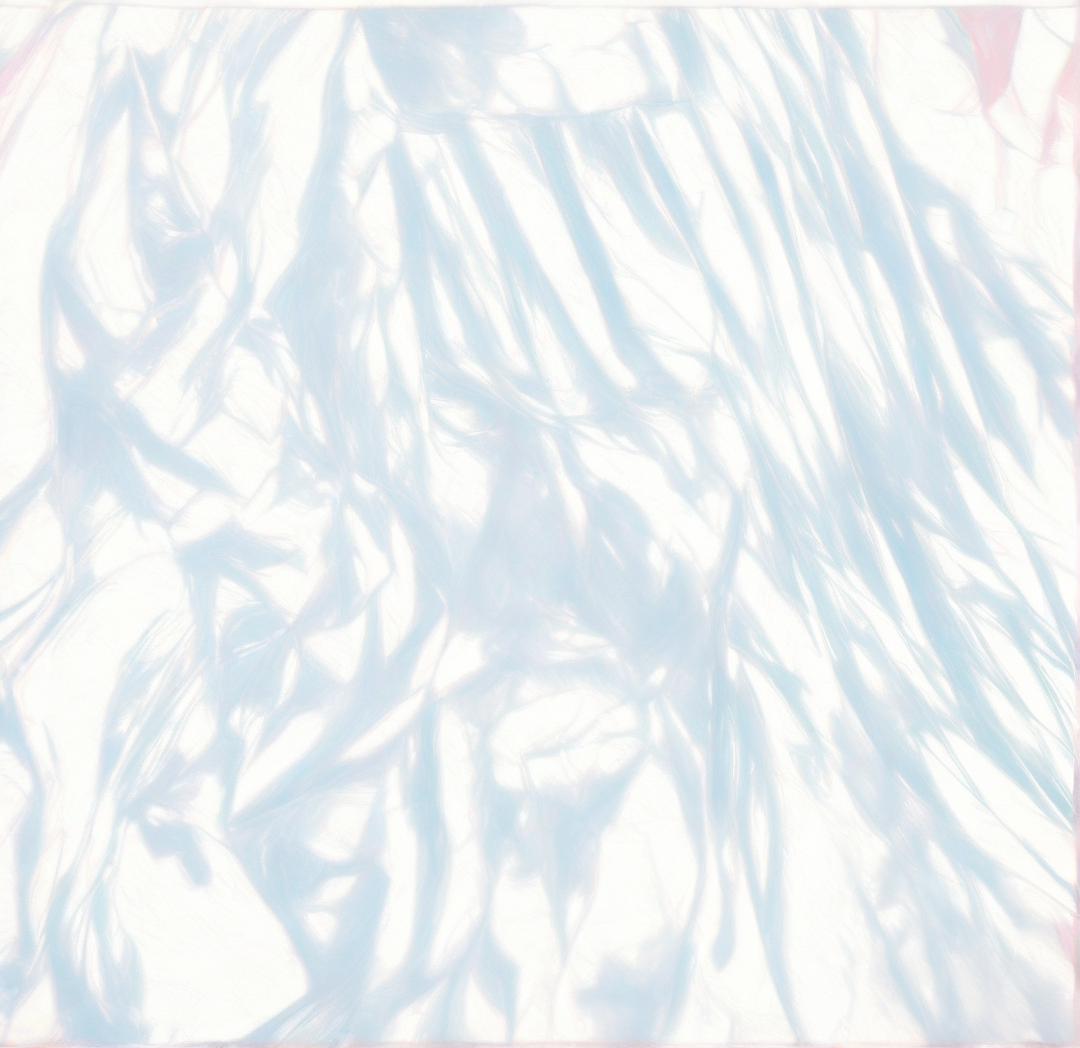
\includegraphics[width=2.0cm]{proc10_adainfalse_gamma1.png} \\[1pt]
\rowlab{10-block}{AdaIN} &

\includegraphics[width=2.0cm]{proc10_adaintrue_gamma0.2.png} &

\includegraphics[width=2.0cm]{proc10_adaintrue_gamma0.4.png} &
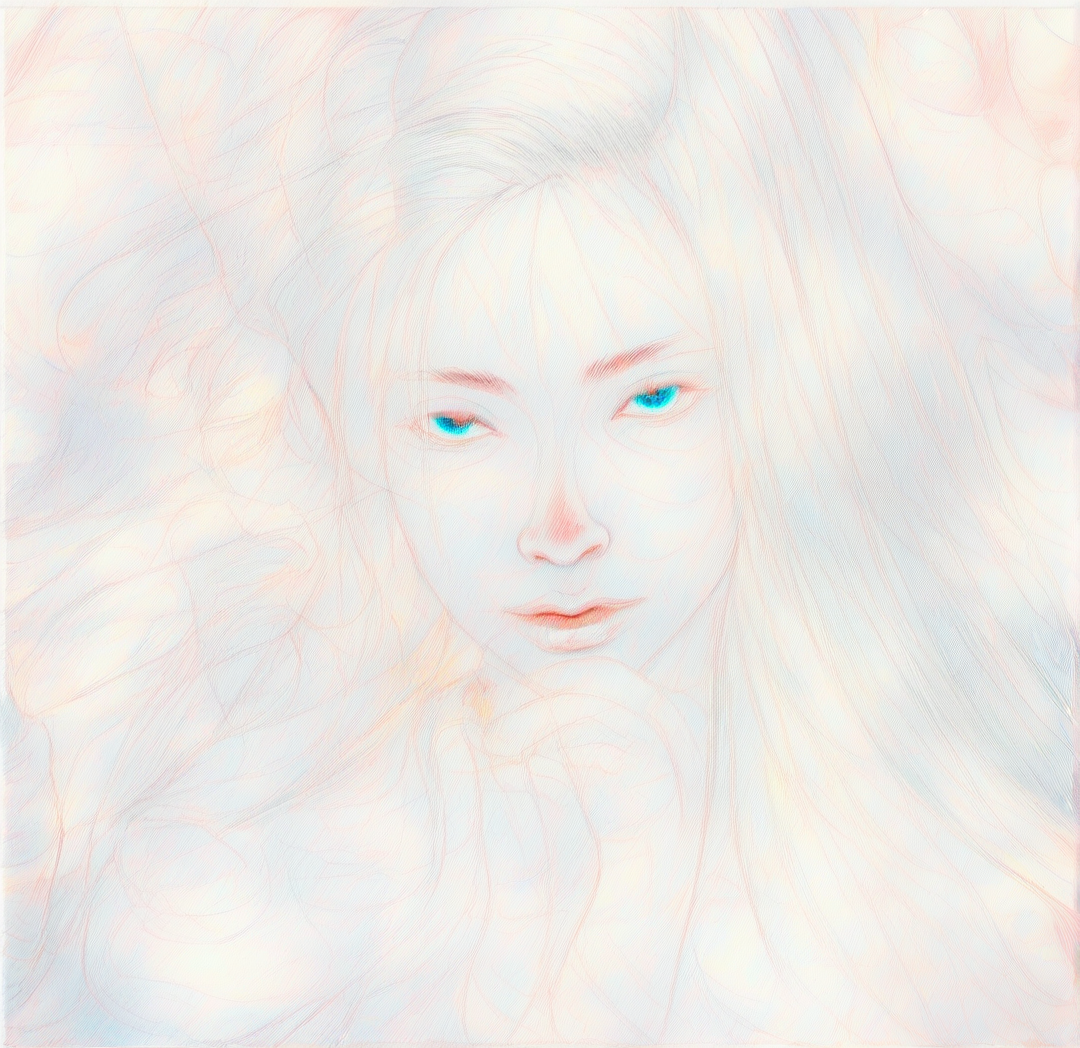
\includegraphics[width=2.0cm]{proc10_adaintrue_gamma0.8.png} &
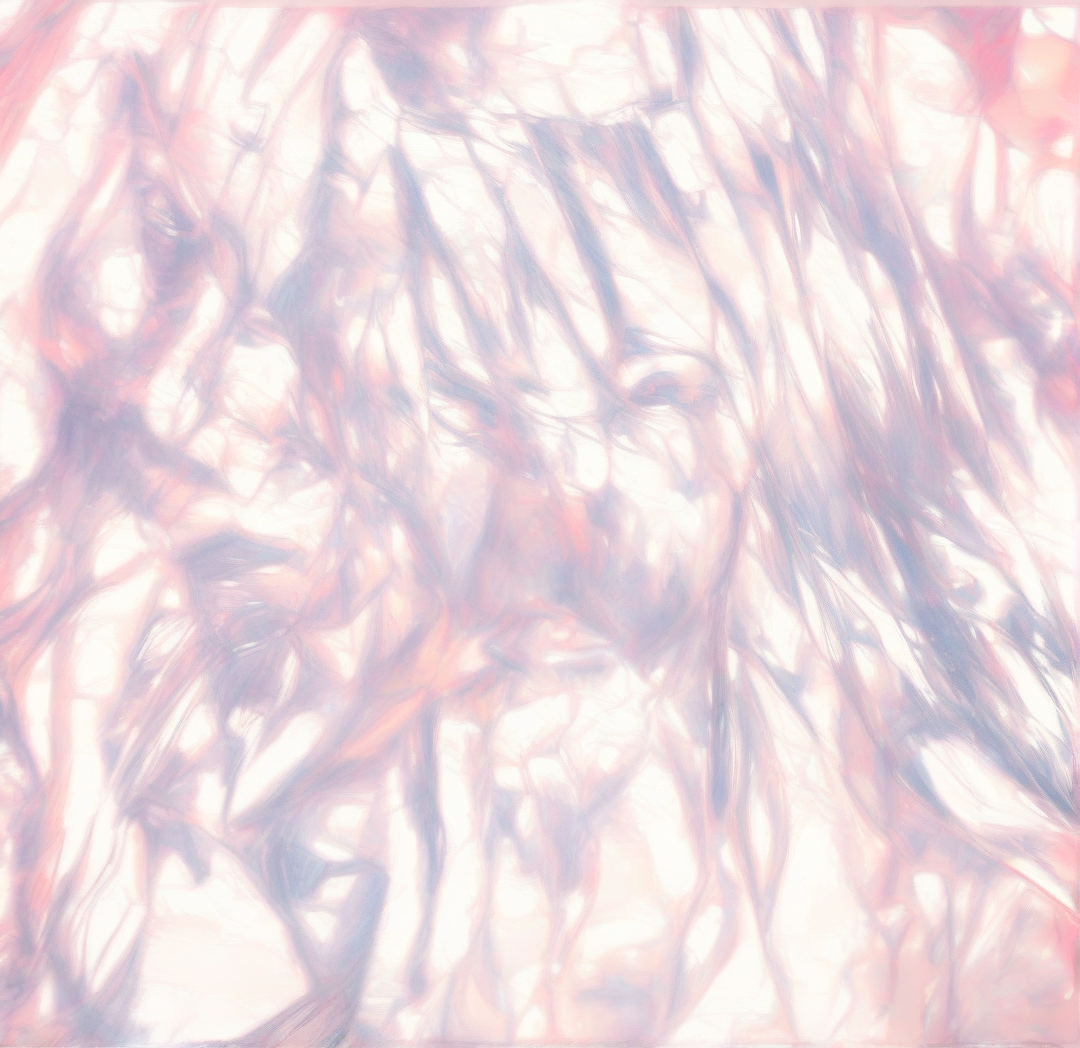
\includegraphics[width=2.0cm]{proc10_adaintrue_gamma1.png} \\
\end{tabular}
\end{document}
